\section{Introduction}\label{s:intro}

We are interested in reconstructing 3D human pose from the observation of single 2D images.
As humans, we have no problem in predicting, at least approximately, the 3D structure of most scenes, including the pose and shape of other people, even from a single view.
However, 2D images notoriously~\citep{Faugeras01geometry} do not contain sufficient geometric information to allow recovery of the third dimension.
Hence, single-view reconstruction is only possible in a probabilistic sense and the goal is to make the posterior distribution as sharp as possible, by learning a strong prior on the space of possible solutions.

Recent progress in single-view 3D pose reconstruction has been impressive.
Methods such as HMR~\citep{kanazawa18end-to-end}, GraphCMR~\citep{kolotouros19convolutional} and SPIN~\citep{kolotouros19learning} formulate this task as learning a deep neural network that maps 2D images to the parameters of a 3D model of the human body, usually SMPL~\cite{loper15smpl}.
These methods work well in general, but not always~(\cref{fig:issues}).
Their main weakness is processing \emph{heavily occluded images} of the object.
When a large part of the object is missing, say the lower body of a sitting human, they output reconstructions that are often implausible.
Since they can produce only one hypothesis as output, they very likely learn to approximate the mean of the posterior distribution, which may not correspond to any plausible pose.
Unfortunately, this failure modality is rather common in applications due to scene clutter and crowds.

In this paper, we propose a solution to this issue.
Specifically, we consider the challenge of recovering 3D mesh reconstructions of complex articulated objects such as humans from highly ambiguous image data, often containing significant occlusions of the object.
Clearly, it is generally impossible to reconstruct the object uniquely if too much evidence is missing; however, we can still predict a \emph{set} containing all possible reconstructions (see \cref{fig:splash}), making this set as small as possible.
While ambiguous pose reconstruction has been previously investigated, as far as we know, this is the first paper that looks specifically at a deep learning approach for ambiguous reconstructions of the \emph{full human mesh}.

% splash
\begin{figure}
\setlength{\fboxsep}{0pt}%
\setlength{\fboxrule}{0pt}%
\centering{\begin{tabular}{@{}c@{}}
    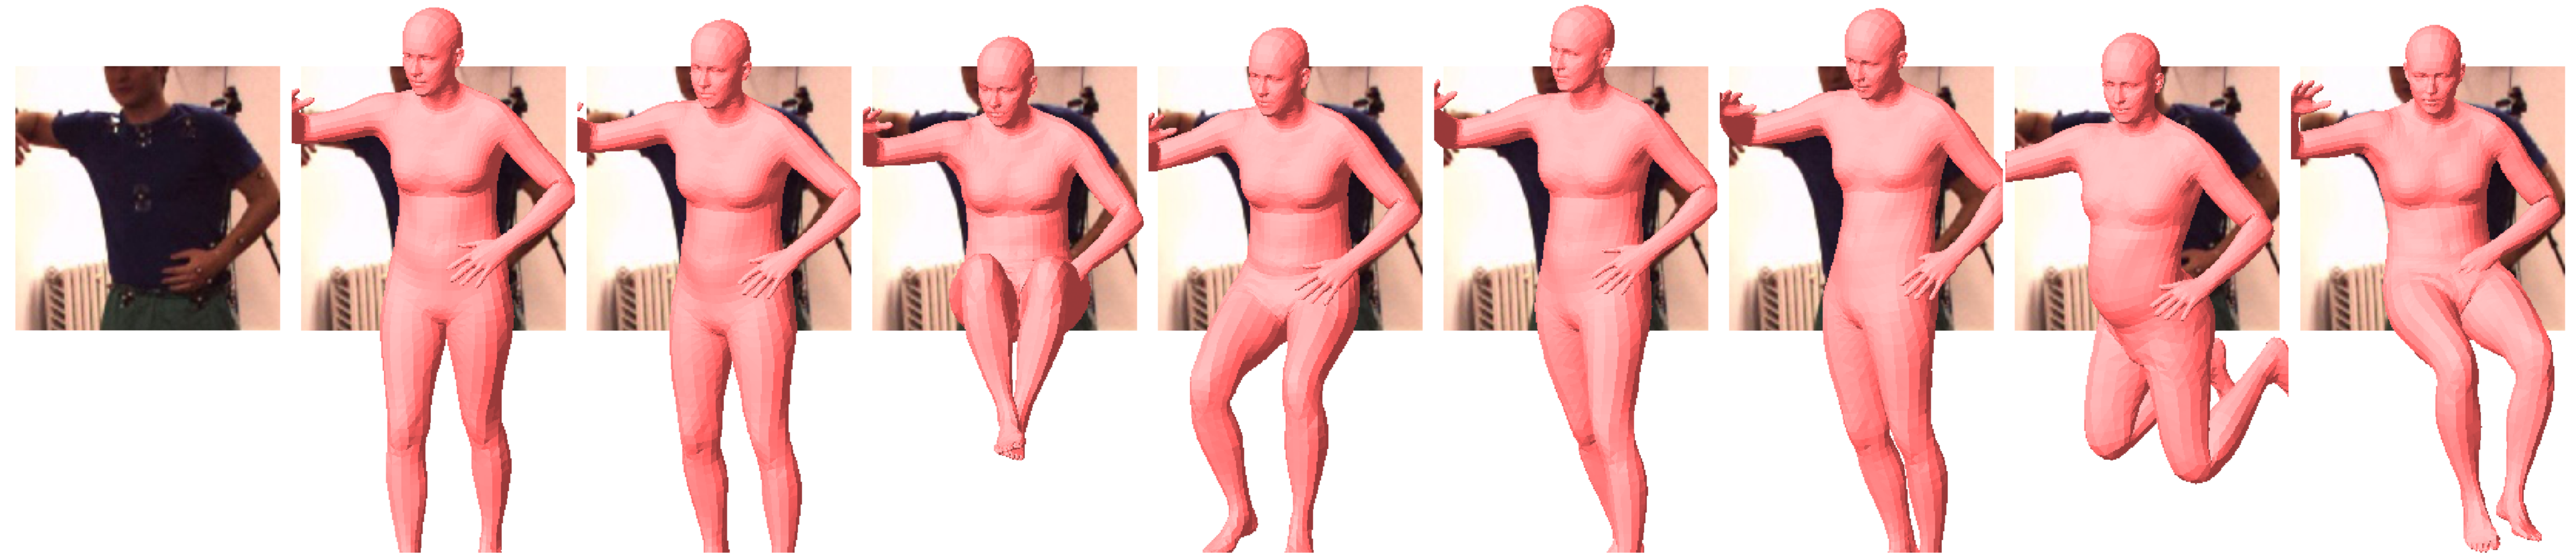
\includegraphics[width=0.49\linewidth,trim=4 8 8 10,clip]{splash/sample_2.pdf} 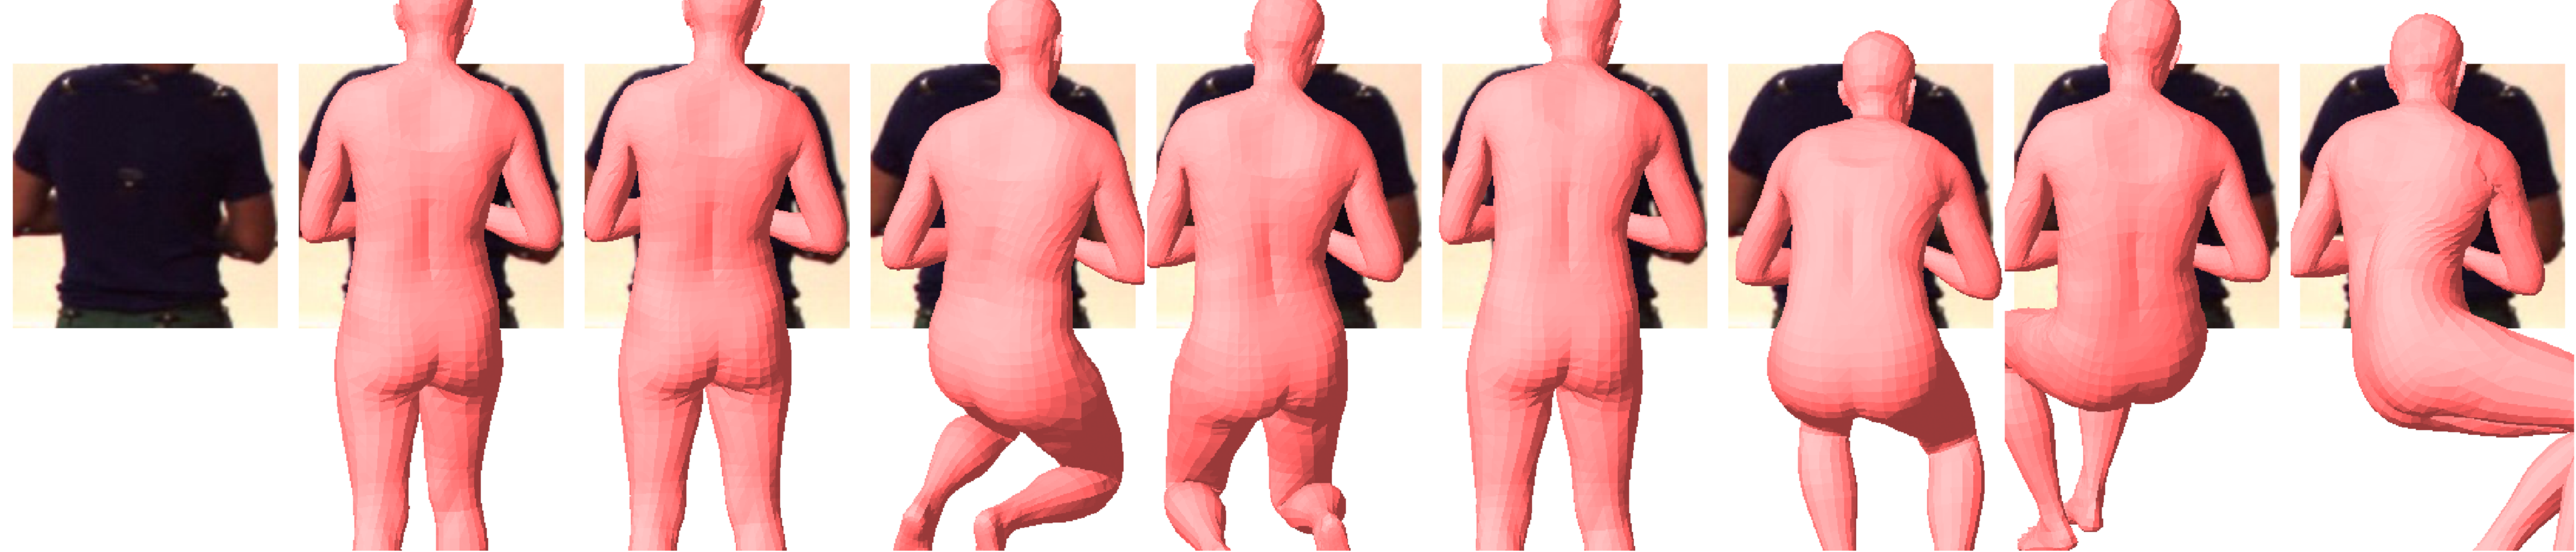
\includegraphics[width=0.49\linewidth,trim=4 8 8 10,clip]{splash/sample_7.pdf}\\
    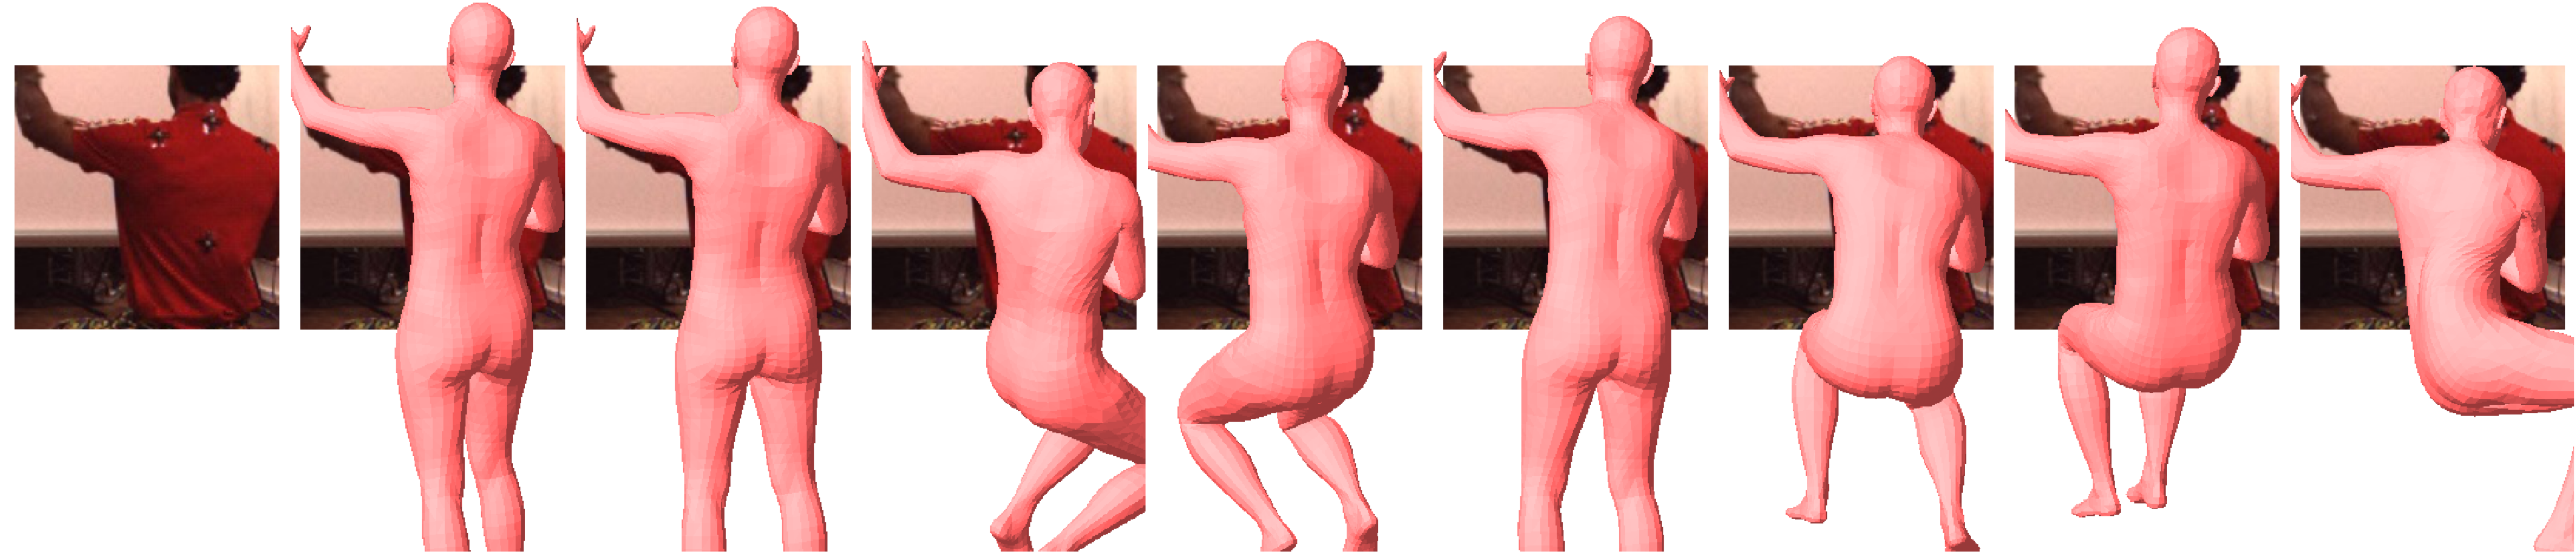
\includegraphics[width=0.49\linewidth,trim=8 10 10 12,clip]{splash/sample_8.pdf} 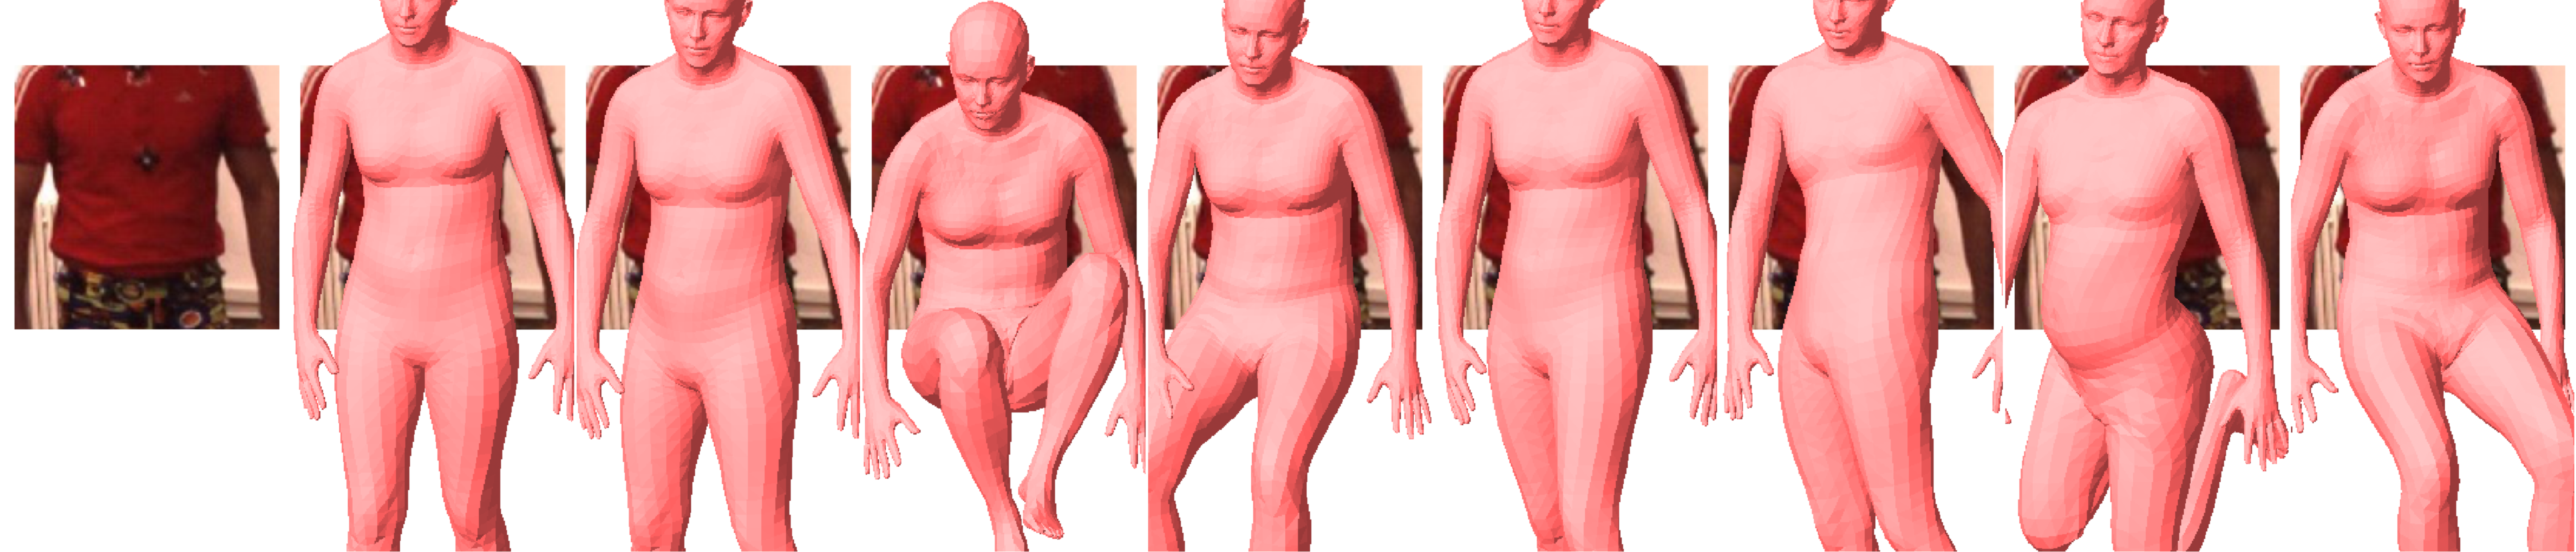
\includegraphics[width=0.49\linewidth,trim=8 10 10  10,clip]{splash/sample_13.pdf}
\end{tabular}}
\vspace{-0.2cm}
\captionof{figure}{
\textbf{Human mesh recovery in an ambiguous setting.}
We propose a novel method that, given an occluded input image of a person, outputs the set of meshes which constitute plausible human bodies that are consistent with the partial view.
The ambiguous poses are predicted using a novel $n$-quantized-best-of-$M$ method.\label{fig:splash}}
% \vspace{-2cm}
\end{figure}

Our primary contribution is to introduce a principled multi-hypothesis framework to model the ambiguities in monocular pose recovery.
In the literature, such multiple-hypotheses networks are often trained with a so-called \emph{best-of-$M$} loss --- namely, during training, the loss is incurred only by the best of the $M$ hypothesis, back-propagating gradients from that alone~\cite{guzman2012multiple}.
In this work we opt for the \emph{best-of-$M$} approach since it has been show to outperform  alternatives (such as variational auto-encoders or mixture density networks) in tasks that are similar to our 3D human pose recovery, and which have constrained output spaces \cite{rupprecht17learning}.

\begin{wrapfigure}{r}{0.4\textwidth}
  \vspace{-0.3cm}
  \begin{center}
    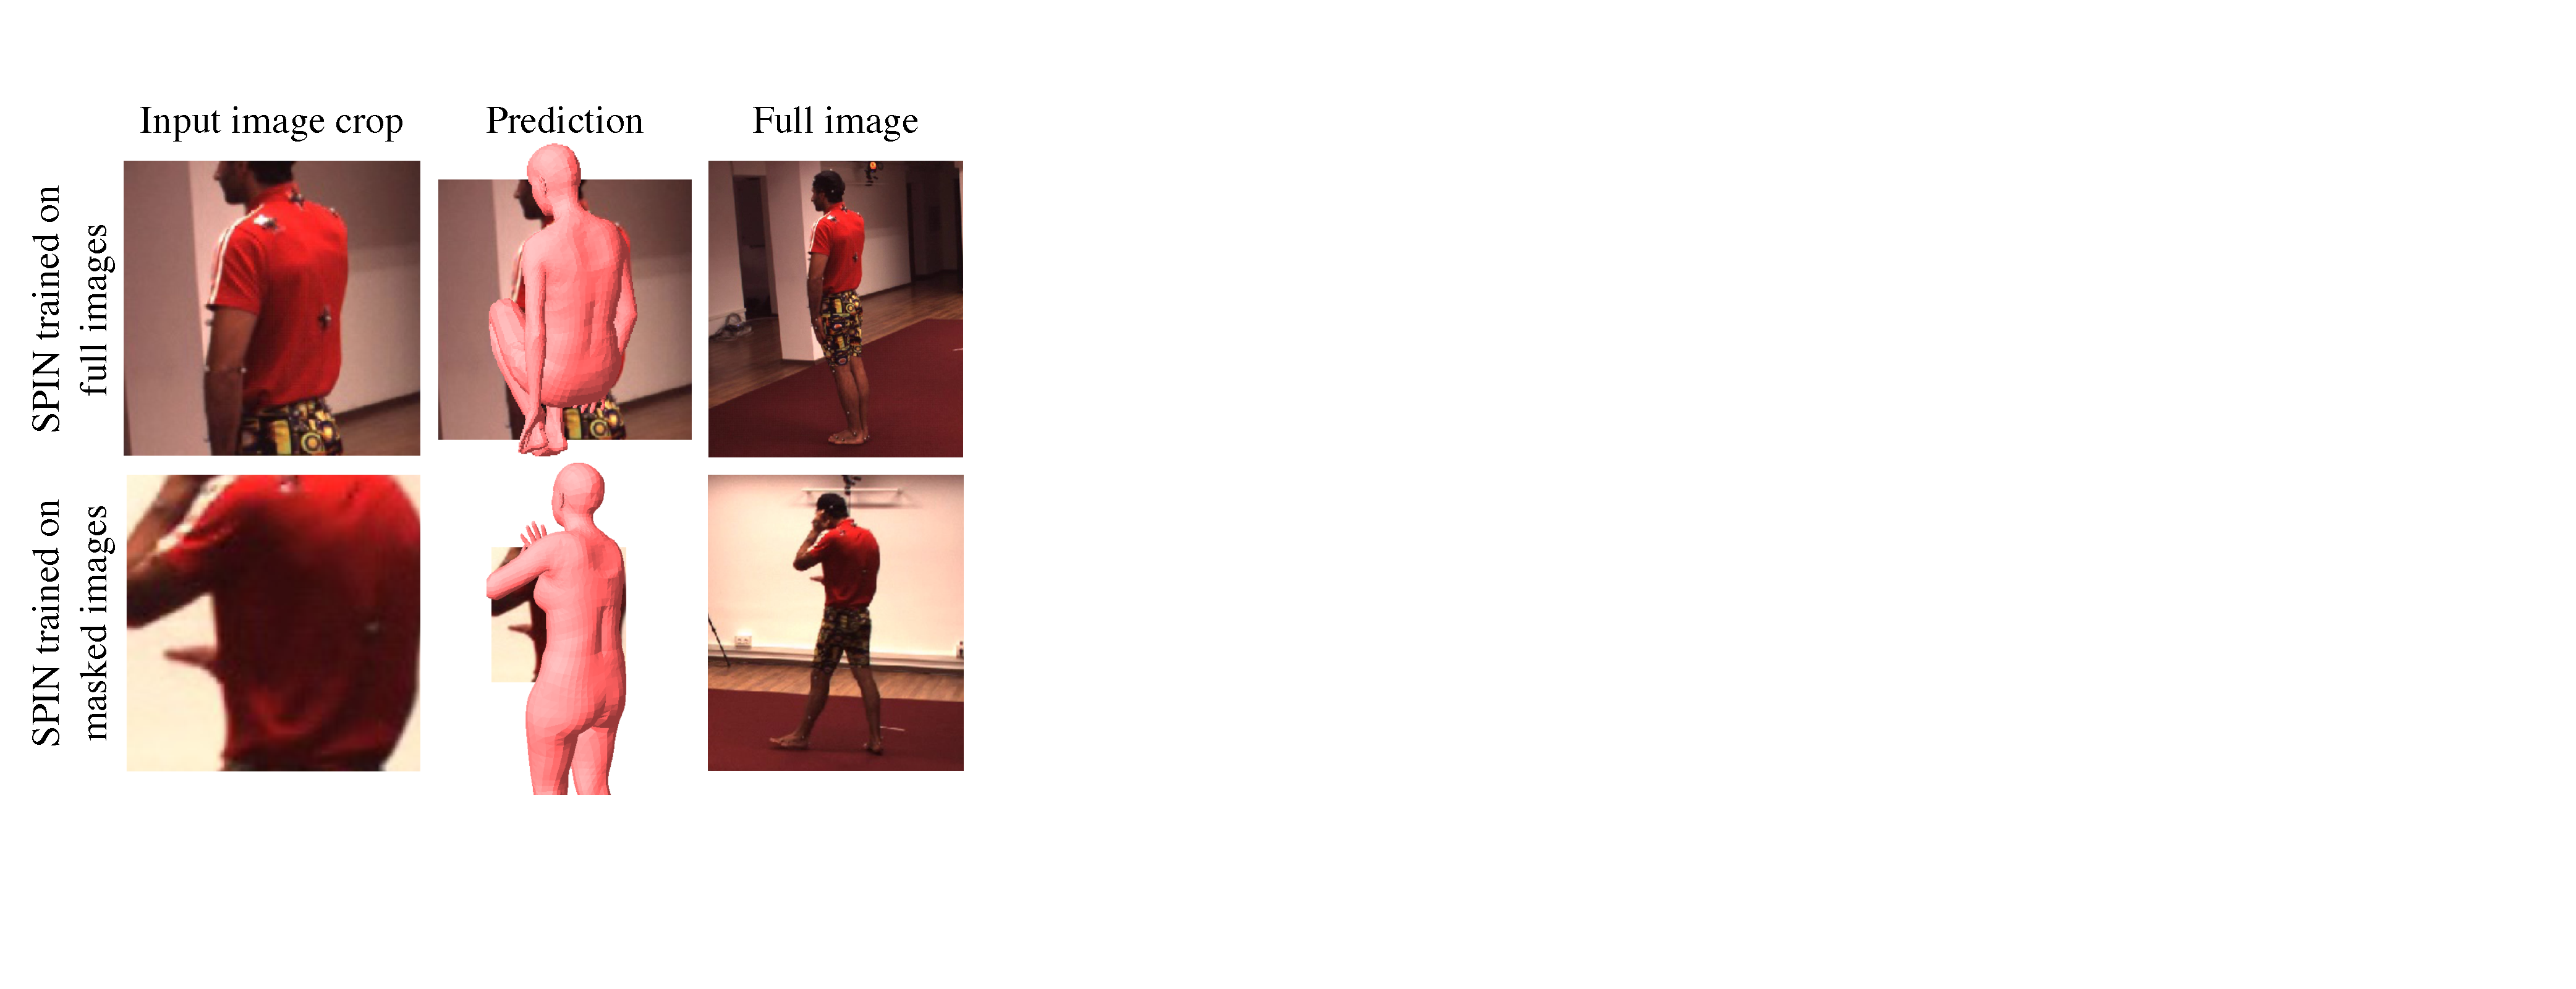
\includegraphics[width=\linewidth]{failures/failure_summary_v2} %
  \end{center}
    \vspace{-0.3cm}
    \caption{\textbf{Top}: Pretrained SPIN model tested on an ambiguous example, \textbf{Bottom}: SPIN model after fine-tuning to ambiguous examples. Note the network tends to regress to the mean over plausible poses, shown by predicting the missing legs vertically downward --- arguably the average position over the training dataset.}\label{fig:issues}
    % \vspace{-0.3cm}
\end{wrapfigure}

% We also make an important contribution to better optimize our multi-hypothesis predictions.

A major drawback of the \emph{best-of-$M$} approach is that it only guarantees that \emph{one} of the hypotheses lies close to the correct solution; however, it says nothing about the plausibility, or lack thereof, of the \emph{other} $M-1$ hypotheses, which can be arbitrarily `bad'.%
%
\footnote{
Theoretically, best-of-$M$ can minimize its loss by quantizing optimally (in the sense of minimum expected distortion) the posterior distribution, which would be desirable for coverage.
However, this is \emph{not} the only solution that optimizes the best-of-$M$ training loss, as in the end it is sufficient that \emph{one} hypothesis per training sample is close to the ground truth.
In fact, this is exactly what happens; for instance, during training hypotheses in best-of-$M$ are known to easily become degenerate and `die off', a clear symptom of this problem.
}
%
Not only does this mean that most of the hypotheses may be uninformative, but in an application we are also unable to tell \emph{which} hypothesis should be used, and we might very well pick a `bad'
one.
% as there is no way of selecting the best one.
This has also a detrimental effect during learning because it  makes gradients sparse as prediction errors are back-propagated only through one of the $M$ hypotheses for each training image.

In order to address these issues, our first contribution is a \emph{hypothesis reprojection loss} that forces each member of the multi-hypothesis set to correctly reproject to 2D image keypoint annotations.
The main benefit is to constrain the \emph{whole} predicted set of meshes to be consistent with the observed image, not just the best hypothesis, also addressing gradient sparsity.

Next, we observe that another drawback of the best-of-{$M$} pipelines is to be tied to a particular value of $M$, whereas in applications we are often interested in tuning the number of hypothesis considered.
Furthermore, minimizing the reprojection loss makes hypotheses geometrically consistent with the observation, but not necessarily likely.
Our second contribution is thus to improve the flexibility of best-of-$M$ models by allowing them to output any smaller number $n<M$ of hypotheses while at the same time making these hypotheses \emph{more representative of likely} poses.
The new method, which we call $n$-quantized-best-of-$M$, does so by quantizing the best-of-$M$ model to output weighed by a \emph{explicit pose prior}, learned by means of normalizing flows.

% In order to do so, since best-of-$M$ lacks an explicit n\emph{prior} over plausible human body poses, thus resulting in an optimal coverage of the \emph{likely} solutions.

%an arbitrary number of $n<M$ hypotheses that optimally cover the set of plausible poses.

% Compared to prior work, we also make a simple but important contribution of modelling ambiguity in the space of 3D model parameters.
% Existing approaches, such as Mixture Density Networks~\cite{bishop94mixture,li19generating}, output instead a distribution on the reconstructed 3D location of a finite set of human body joints.
% This is straightforward, but difficult to extend to full 3D meshes.
% Instead, we argue that the parameters of the 3D model offer a better space for coding not just 3D shapes and poses, but also their ambiguities.
% As far as we could determine, we are the first to model ambiguous reconstructions directly in the space of human body model parameters.

To summarise, our key contributions are as follows.
First, we deal with the challenge of 3D mesh reconstruction for articulated objects such as humans in \emph{ambiguous} scenarios.
Second, we introduce a \emph{$n$-quantized-best-of-$M$} mechanism to allow best-of-$M$ models to generate an arbitrary number of $n<M$ predictions.
Third, we introduce a mode-wise re-projection loss for multi-hypothesis prediction, to ensure that predicted hypotheses are \emph{all} consistent with the input.

Empirically, we achieve state-of-the-art monocular mesh recovery accuracy on Human36M, its more challenging version augmented with heavy occlusions, and the 3DPW datasets.
Our ablation study validates each of our modelling choices, demonstrating their positive effect.
